% Options for packages loaded elsewhere
\PassOptionsToPackage{unicode}{hyperref}
\PassOptionsToPackage{hyphens}{url}
\PassOptionsToPackage{dvipsnames,svgnames,x11names}{xcolor}
%
\documentclass[
  letterpaper,
  DIV=11,
  numbers=noendperiod]{scrreprt}

\usepackage{amsmath,amssymb}
\usepackage{iftex}
\ifPDFTeX
  \usepackage[T1]{fontenc}
  \usepackage[utf8]{inputenc}
  \usepackage{textcomp} % provide euro and other symbols
\else % if luatex or xetex
  \usepackage{unicode-math}
  \defaultfontfeatures{Scale=MatchLowercase}
  \defaultfontfeatures[\rmfamily]{Ligatures=TeX,Scale=1}
\fi
\usepackage{lmodern}
\ifPDFTeX\else  
    % xetex/luatex font selection
\fi
% Use upquote if available, for straight quotes in verbatim environments
\IfFileExists{upquote.sty}{\usepackage{upquote}}{}
\IfFileExists{microtype.sty}{% use microtype if available
  \usepackage[]{microtype}
  \UseMicrotypeSet[protrusion]{basicmath} % disable protrusion for tt fonts
}{}
\makeatletter
\@ifundefined{KOMAClassName}{% if non-KOMA class
  \IfFileExists{parskip.sty}{%
    \usepackage{parskip}
  }{% else
    \setlength{\parindent}{0pt}
    \setlength{\parskip}{6pt plus 2pt minus 1pt}}
}{% if KOMA class
  \KOMAoptions{parskip=half}}
\makeatother
\usepackage{xcolor}
\setlength{\emergencystretch}{3em} % prevent overfull lines
\setcounter{secnumdepth}{5}
% Make \paragraph and \subparagraph free-standing
\ifx\paragraph\undefined\else
  \let\oldparagraph\paragraph
  \renewcommand{\paragraph}[1]{\oldparagraph{#1}\mbox{}}
\fi
\ifx\subparagraph\undefined\else
  \let\oldsubparagraph\subparagraph
  \renewcommand{\subparagraph}[1]{\oldsubparagraph{#1}\mbox{}}
\fi

\usepackage{color}
\usepackage{fancyvrb}
\newcommand{\VerbBar}{|}
\newcommand{\VERB}{\Verb[commandchars=\\\{\}]}
\DefineVerbatimEnvironment{Highlighting}{Verbatim}{commandchars=\\\{\}}
% Add ',fontsize=\small' for more characters per line
\usepackage{framed}
\definecolor{shadecolor}{RGB}{241,243,245}
\newenvironment{Shaded}{\begin{snugshade}}{\end{snugshade}}
\newcommand{\AlertTok}[1]{\textcolor[rgb]{0.68,0.00,0.00}{#1}}
\newcommand{\AnnotationTok}[1]{\textcolor[rgb]{0.37,0.37,0.37}{#1}}
\newcommand{\AttributeTok}[1]{\textcolor[rgb]{0.40,0.45,0.13}{#1}}
\newcommand{\BaseNTok}[1]{\textcolor[rgb]{0.68,0.00,0.00}{#1}}
\newcommand{\BuiltInTok}[1]{\textcolor[rgb]{0.00,0.23,0.31}{#1}}
\newcommand{\CharTok}[1]{\textcolor[rgb]{0.13,0.47,0.30}{#1}}
\newcommand{\CommentTok}[1]{\textcolor[rgb]{0.37,0.37,0.37}{#1}}
\newcommand{\CommentVarTok}[1]{\textcolor[rgb]{0.37,0.37,0.37}{\textit{#1}}}
\newcommand{\ConstantTok}[1]{\textcolor[rgb]{0.56,0.35,0.01}{#1}}
\newcommand{\ControlFlowTok}[1]{\textcolor[rgb]{0.00,0.23,0.31}{#1}}
\newcommand{\DataTypeTok}[1]{\textcolor[rgb]{0.68,0.00,0.00}{#1}}
\newcommand{\DecValTok}[1]{\textcolor[rgb]{0.68,0.00,0.00}{#1}}
\newcommand{\DocumentationTok}[1]{\textcolor[rgb]{0.37,0.37,0.37}{\textit{#1}}}
\newcommand{\ErrorTok}[1]{\textcolor[rgb]{0.68,0.00,0.00}{#1}}
\newcommand{\ExtensionTok}[1]{\textcolor[rgb]{0.00,0.23,0.31}{#1}}
\newcommand{\FloatTok}[1]{\textcolor[rgb]{0.68,0.00,0.00}{#1}}
\newcommand{\FunctionTok}[1]{\textcolor[rgb]{0.28,0.35,0.67}{#1}}
\newcommand{\ImportTok}[1]{\textcolor[rgb]{0.00,0.46,0.62}{#1}}
\newcommand{\InformationTok}[1]{\textcolor[rgb]{0.37,0.37,0.37}{#1}}
\newcommand{\KeywordTok}[1]{\textcolor[rgb]{0.00,0.23,0.31}{#1}}
\newcommand{\NormalTok}[1]{\textcolor[rgb]{0.00,0.23,0.31}{#1}}
\newcommand{\OperatorTok}[1]{\textcolor[rgb]{0.37,0.37,0.37}{#1}}
\newcommand{\OtherTok}[1]{\textcolor[rgb]{0.00,0.23,0.31}{#1}}
\newcommand{\PreprocessorTok}[1]{\textcolor[rgb]{0.68,0.00,0.00}{#1}}
\newcommand{\RegionMarkerTok}[1]{\textcolor[rgb]{0.00,0.23,0.31}{#1}}
\newcommand{\SpecialCharTok}[1]{\textcolor[rgb]{0.37,0.37,0.37}{#1}}
\newcommand{\SpecialStringTok}[1]{\textcolor[rgb]{0.13,0.47,0.30}{#1}}
\newcommand{\StringTok}[1]{\textcolor[rgb]{0.13,0.47,0.30}{#1}}
\newcommand{\VariableTok}[1]{\textcolor[rgb]{0.07,0.07,0.07}{#1}}
\newcommand{\VerbatimStringTok}[1]{\textcolor[rgb]{0.13,0.47,0.30}{#1}}
\newcommand{\WarningTok}[1]{\textcolor[rgb]{0.37,0.37,0.37}{\textit{#1}}}

\providecommand{\tightlist}{%
  \setlength{\itemsep}{0pt}\setlength{\parskip}{0pt}}\usepackage{longtable,booktabs,array}
\usepackage{calc} % for calculating minipage widths
% Correct order of tables after \paragraph or \subparagraph
\usepackage{etoolbox}
\makeatletter
\patchcmd\longtable{\par}{\if@noskipsec\mbox{}\fi\par}{}{}
\makeatother
% Allow footnotes in longtable head/foot
\IfFileExists{footnotehyper.sty}{\usepackage{footnotehyper}}{\usepackage{footnote}}
\makesavenoteenv{longtable}
\usepackage{graphicx}
\makeatletter
\def\maxwidth{\ifdim\Gin@nat@width>\linewidth\linewidth\else\Gin@nat@width\fi}
\def\maxheight{\ifdim\Gin@nat@height>\textheight\textheight\else\Gin@nat@height\fi}
\makeatother
% Scale images if necessary, so that they will not overflow the page
% margins by default, and it is still possible to overwrite the defaults
% using explicit options in \includegraphics[width, height, ...]{}
\setkeys{Gin}{width=\maxwidth,height=\maxheight,keepaspectratio}
% Set default figure placement to htbp
\makeatletter
\def\fps@figure{htbp}
\makeatother
% definitions for citeproc citations
\NewDocumentCommand\citeproctext{}{}
\NewDocumentCommand\citeproc{mm}{%
  \begingroup\def\citeproctext{#2}\cite{#1}\endgroup}
\makeatletter
 % allow citations to break across lines
 \let\@cite@ofmt\@firstofone
 % avoid brackets around text for \cite:
 \def\@biblabel#1{}
 \def\@cite#1#2{{#1\if@tempswa , #2\fi}}
\makeatother
\newlength{\cslhangindent}
\setlength{\cslhangindent}{1.5em}
\newlength{\csllabelwidth}
\setlength{\csllabelwidth}{3em}
\newenvironment{CSLReferences}[2] % #1 hanging-indent, #2 entry-spacing
 {\begin{list}{}{%
  \setlength{\itemindent}{0pt}
  \setlength{\leftmargin}{0pt}
  \setlength{\parsep}{0pt}
  % turn on hanging indent if param 1 is 1
  \ifodd #1
   \setlength{\leftmargin}{\cslhangindent}
   \setlength{\itemindent}{-1\cslhangindent}
  \fi
  % set entry spacing
  \setlength{\itemsep}{#2\baselineskip}}}
 {\end{list}}
\usepackage{calc}
\newcommand{\CSLBlock}[1]{\hfill\break\parbox[t]{\linewidth}{\strut\ignorespaces#1\strut}}
\newcommand{\CSLLeftMargin}[1]{\parbox[t]{\csllabelwidth}{\strut#1\strut}}
\newcommand{\CSLRightInline}[1]{\parbox[t]{\linewidth - \csllabelwidth}{\strut#1\strut}}
\newcommand{\CSLIndent}[1]{\hspace{\cslhangindent}#1}

\KOMAoption{captions}{tableheading}
\makeatletter
\@ifpackageloaded{tcolorbox}{}{\usepackage[skins,breakable]{tcolorbox}}
\@ifpackageloaded{fontawesome5}{}{\usepackage{fontawesome5}}
\definecolor{quarto-callout-color}{HTML}{909090}
\definecolor{quarto-callout-note-color}{HTML}{0758E5}
\definecolor{quarto-callout-important-color}{HTML}{CC1914}
\definecolor{quarto-callout-warning-color}{HTML}{EB9113}
\definecolor{quarto-callout-tip-color}{HTML}{00A047}
\definecolor{quarto-callout-caution-color}{HTML}{FC5300}
\definecolor{quarto-callout-color-frame}{HTML}{acacac}
\definecolor{quarto-callout-note-color-frame}{HTML}{4582ec}
\definecolor{quarto-callout-important-color-frame}{HTML}{d9534f}
\definecolor{quarto-callout-warning-color-frame}{HTML}{f0ad4e}
\definecolor{quarto-callout-tip-color-frame}{HTML}{02b875}
\definecolor{quarto-callout-caution-color-frame}{HTML}{fd7e14}
\makeatother
\makeatletter
\@ifpackageloaded{bookmark}{}{\usepackage{bookmark}}
\makeatother
\makeatletter
\@ifpackageloaded{caption}{}{\usepackage{caption}}
\AtBeginDocument{%
\ifdefined\contentsname
  \renewcommand*\contentsname{Tabla de contenidos}
\else
  \newcommand\contentsname{Tabla de contenidos}
\fi
\ifdefined\listfigurename
  \renewcommand*\listfigurename{Listado de Figuras}
\else
  \newcommand\listfigurename{Listado de Figuras}
\fi
\ifdefined\listtablename
  \renewcommand*\listtablename{Listado de Tablas}
\else
  \newcommand\listtablename{Listado de Tablas}
\fi
\ifdefined\figurename
  \renewcommand*\figurename{Figura}
\else
  \newcommand\figurename{Figura}
\fi
\ifdefined\tablename
  \renewcommand*\tablename{Tabla}
\else
  \newcommand\tablename{Tabla}
\fi
}
\@ifpackageloaded{float}{}{\usepackage{float}}
\floatstyle{ruled}
\@ifundefined{c@chapter}{\newfloat{codelisting}{h}{lop}}{\newfloat{codelisting}{h}{lop}[chapter]}
\floatname{codelisting}{Listado}
\newcommand*\listoflistings{\listof{codelisting}{Listado de Listados}}
\makeatother
\makeatletter
\makeatother
\makeatletter
\@ifpackageloaded{caption}{}{\usepackage{caption}}
\@ifpackageloaded{subcaption}{}{\usepackage{subcaption}}
\makeatother
\ifLuaTeX
\usepackage[bidi=basic]{babel}
\else
\usepackage[bidi=default]{babel}
\fi
\babelprovide[main,import]{spanish}
% get rid of language-specific shorthands (see #6817):
\let\LanguageShortHands\languageshorthands
\def\languageshorthands#1{}
\ifLuaTeX
  \usepackage{selnolig}  % disable illegal ligatures
\fi
\usepackage{bookmark}

\IfFileExists{xurl.sty}{\usepackage{xurl}}{} % add URL line breaks if available
\urlstyle{same} % disable monospaced font for URLs
\hypersetup{
  pdftitle={Matemáticas y Estadística Farmacia},
  pdfauthor={Alirio Cruz; Irene García},
  pdflang={es},
  colorlinks=true,
  linkcolor={blue},
  filecolor={Maroon},
  citecolor={Blue},
  urlcolor={Blue},
  pdfcreator={LaTeX via pandoc}}

\title{Matemáticas y Estadística Farmacia}
\author{Alirio Cruz \and Irene García}
\date{2024-09-11}

\begin{document}
\maketitle

\renewcommand*\contentsname{Tabla de contenidos}
{
\hypersetup{linkcolor=}
\setcounter{tocdepth}{2}
\tableofcontents
}
\bookmarksetup{startatroot}

\chapter*{Presentación}\label{presentaciuxf3n}
\addcontentsline{toc}{chapter}{Presentación}

\markboth{Presentación}{Presentación}

Esto es una edición en línea de los apuntes de la asignatura de
Matemáticas y Estadística.

El enfoque es teórico-práctico para el grado de Farmacia de la UIB.

\bookmarksetup{startatroot}

\chapter{Matemáticas básicas}\label{matemuxe1ticas-buxe1sicas}

En este primer tema, empezaremos por instalar el software necesario para
el análisis estadístico y la visualización de datos, y luego revisaremos
los conceptos básicos de funciones lineales, exponenciales, logarítmicas
y polinómicas, que son fundamentales para modelar y analizar fenómenos
farmacéuticos. Todo estos conocimientos son cruciales para realizar
cálculos precisos de dosis, desarrollar y evaluar nuevos medicamentos,
así como para llevar a cabo estudios de bioequivalencia y análisis de
farmacoeconomía.

\section{R y Jamovi}\label{r-y-jamovi}

Es fundamental utilizar un software especializado que simplifique la
resolución de problemas y optimice el análisis estadístico de datos.
Estas herramientas no solo agilizan los cálculos y procesamientos
complejos, sino que también mejoran la precisión y fiabilidad de los
resultados obtenidos. Además, permiten una redacción más clara y
estructurada de informes, facilitando la presentación de resultados de
manera profesional y efectiva.

En este curso utilizaremos el software \texttt{jamovi} (interfaz gráfica
que emplea como base R). \texttt{R} es un entorno de programación
estadística de código abierto que ofrece una amplia gama de funciones y
paquetes para el análisis de datos y la generación de gráficos.
\texttt{Jamovi} es una herramienta más accesible que nos permitirá
centrarnos en el análisis y la interpretación de datos, en lugar de en
la sintaxis de programación.

Instalar R es muy sencillo; pero es conveniente que dispongáis de su
versión más reciente y que regularmente lo pongáis al día. Los pasos a
realizar en Windows o Mac OS X para instalar su última versión son los
siguientes:

\begin{itemize}
\item
  Si sois usuarios de Windows, acceded a la página web de la
  \href{http://cran.r-project.org/}{\emph{CRAN}} y pulsad sobre el
  enlace \emph{Download R for Windows}. A continuación, entrad en el
  enlace \emph{base}, descargad R y seguid las instrucciones de
  instalación del documento \emph{Installation and other instructions}
  que encontraréis en esa misma página.
\item
  Si sois usuarios de Mac OS X, acceded a la página web de la
  \href{http://cran.r-project.org/}{\emph{CRAN}} y pulsad sobre el
  enlace \emph{Download R for Mac OS X}. A continuación, descargad el
  fichero \texttt{.pkg} correspondiente y, una vez descargado, abridlo y
  seguid las instrucciones del Asistente de Instalación.
\item
  Si trabajáis con Ubuntu o Debian, para instalar la última versión de R
  basta que ejecutéis en una terminal, estando conectados a Internet, la
  siguiente instrucción:
\end{itemize}

\begin{verbatim}
sudo aptitude install r-base
\end{verbatim}

Cuando instaláis R para Windows o Mac OS X, con él también se os instala
una interfaz gráfica que se abrirá al abrir la aplicación y en la que
podréis trabajar.

\begin{center}
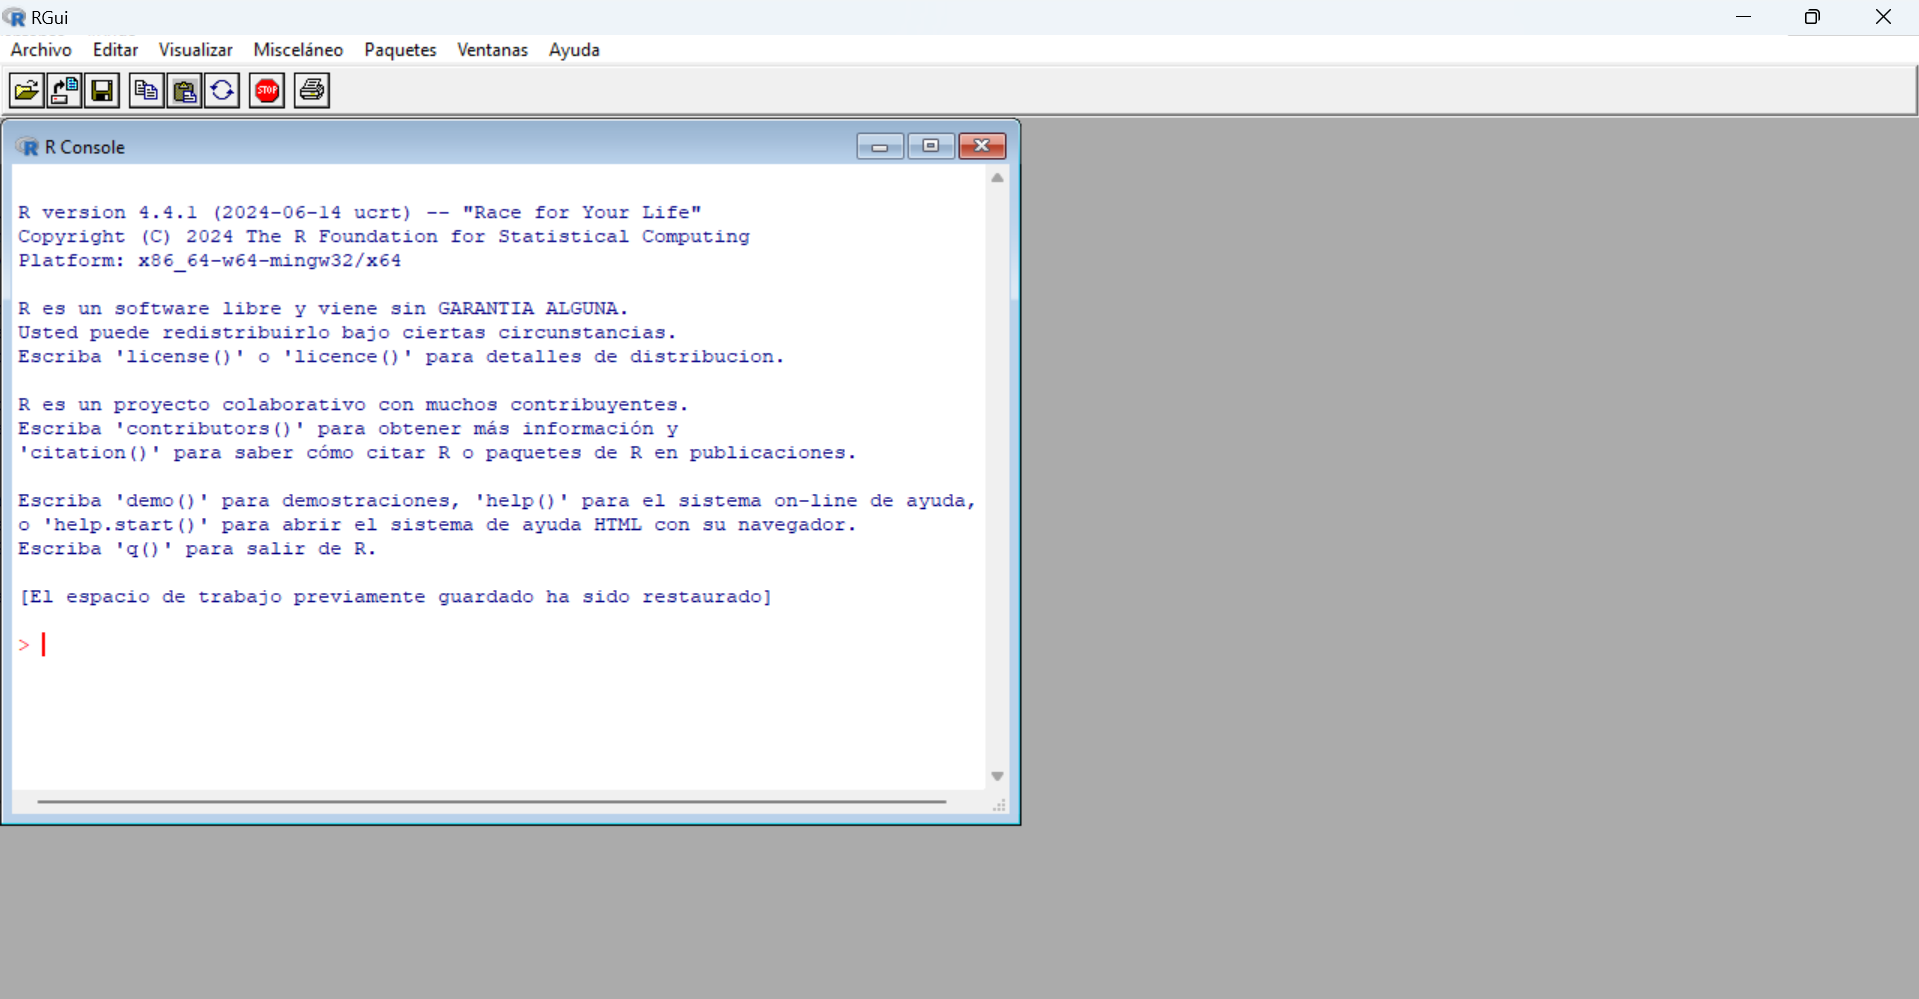
\includegraphics[width=0.8\textwidth,height=\textheight]{Figuras/RTerminal.png}
\end{center}

La instalación para Linux no lleva una interfaz por defecto, así que sus
usuarios tienen que trabajar con R en la terminal (ejecutando R para
iniciar una sesión) o instalar aparte una interfaz. Independientemente
de todas estas posibilidades, en este curso usaremos \emph{RStudio} como
interfaz gráfica de usuario de R para todos los sistemas operativos.

\begin{tcolorbox}[enhanced jigsaw, colframe=quarto-callout-note-color-frame, coltitle=black, colback=white, toptitle=1mm, bottomrule=.15mm, bottomtitle=1mm, leftrule=.75mm, opacityback=0, rightrule=.15mm, titlerule=0mm, title=\textcolor{quarto-callout-note-color}{\faInfo}\hspace{0.5em}{Nota}, arc=.35mm, toprule=.15mm, left=2mm, opacitybacktitle=0.6, breakable, colbacktitle=quarto-callout-note-color!10!white]

R version 4.4.1 (2024-06-14 ucrt) -- ``Race for Your Life'' Copyright
(C) 2024 The R Foundation for Statistical Computing Platform:
x86\_64-w64-mingw32/x64

R es un software libre y viene sin GARANTIA ALGUNA. Usted puede
redistribuirlo bajo ciertas circunstancias. Escriba `license()' o
`licence()' para detalles de distribucion.

R es un proyecto colaborativo con muchos contribuyentes. Escriba
`contributors()' para obtener más información y `citation()' para saber
cómo citar R o paquetes de R en publicaciones.

Escriba `demo()' para demostraciones, `help()' para el sistema on-line
de ayuda, o `help.start()' para abrir el sistema de ayuda HTML con su
navegador. Escriba `q()' para salir de R.

\end{tcolorbox}

\begin{center}

\includegraphics[width=0.4\textwidth,height=\textheight]{Figuras/MM1.jpg}
\end{center}

Para que nuestra interfaz con R sea agradable, podemos usar varias
aplicaciones disponibles, como \texttt{Rstudio},
\texttt{Visual\ Studio\ Code} o \texttt{Jamovi}. Por facilidad usaremos
\texttt{Jamovi}

\subsection{Instalación de Jamovi}\label{instalaciuxf3n-de-jamovi}

Según la pagina de \href{https://www.jamovi.org/}{Jamovi}, y en una
traducción al castellano usando Google translate obtenemos:

\begin{itemize}
\item
  Estadísticas simplificadas: Jamovi es una nueva hoja de cálculo
  estadística de ``tercera generación''. Diseñada desde cero para que
  sea fácil de usar, Jamovi es una alternativa atractiva a productos
  estadísticos costosos como SPSS y SAS.
\item
  Integración con R: Jamovi está construido sobre el lenguaje
  estadístico R, lo que le brinda acceso a lo mejor que la comunidad
  estadística tiene para ofrecer. ¿Le gustaría el código R para sus
  análisis? Jamovi también puede proporcionárselo.
\item
  Gratuito y abierto: Jamovi siempre será gratuito y abierto: ese es uno
  de nuestros valores fundamentales, porque Jamovi está hecho por la
  comunidad científica, para la comunidad científica.
\end{itemize}

Adicional a esto, instalaremos el software, siguiendo las instrucciones
que aparecen en el botón \textbf{Download and install jamovi onto your
computer}

Luego de la instalación debe aparecer en su busqueda de windows.
\begin{center}
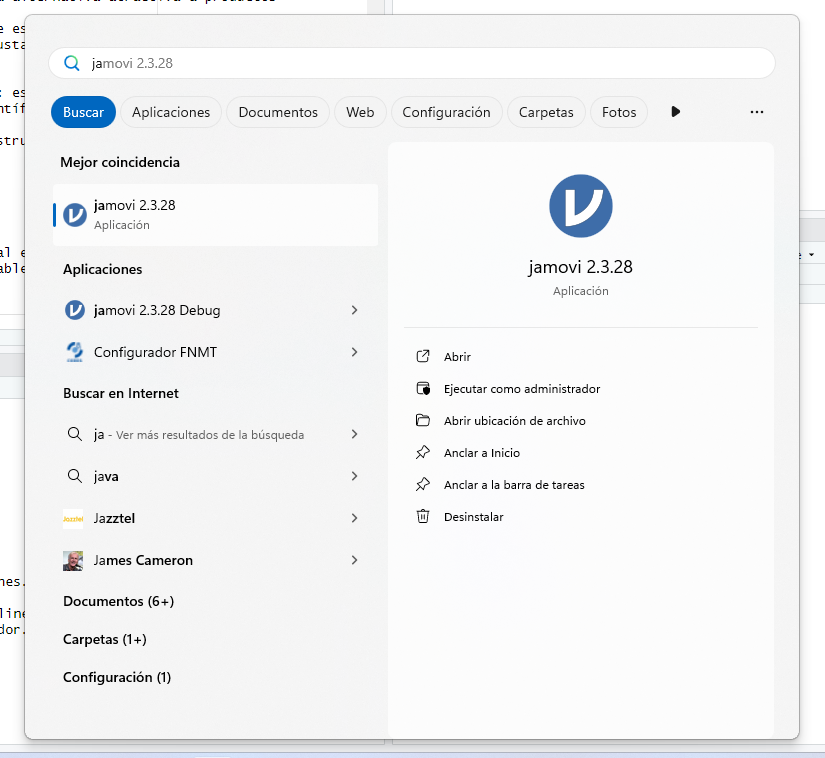
\includegraphics[width=0.5\textwidth,height=\textheight]{Figuras/JAM1.png}
\end{center}

Y nos aparecerá esta interfaz para trabajar.

\begin{center}
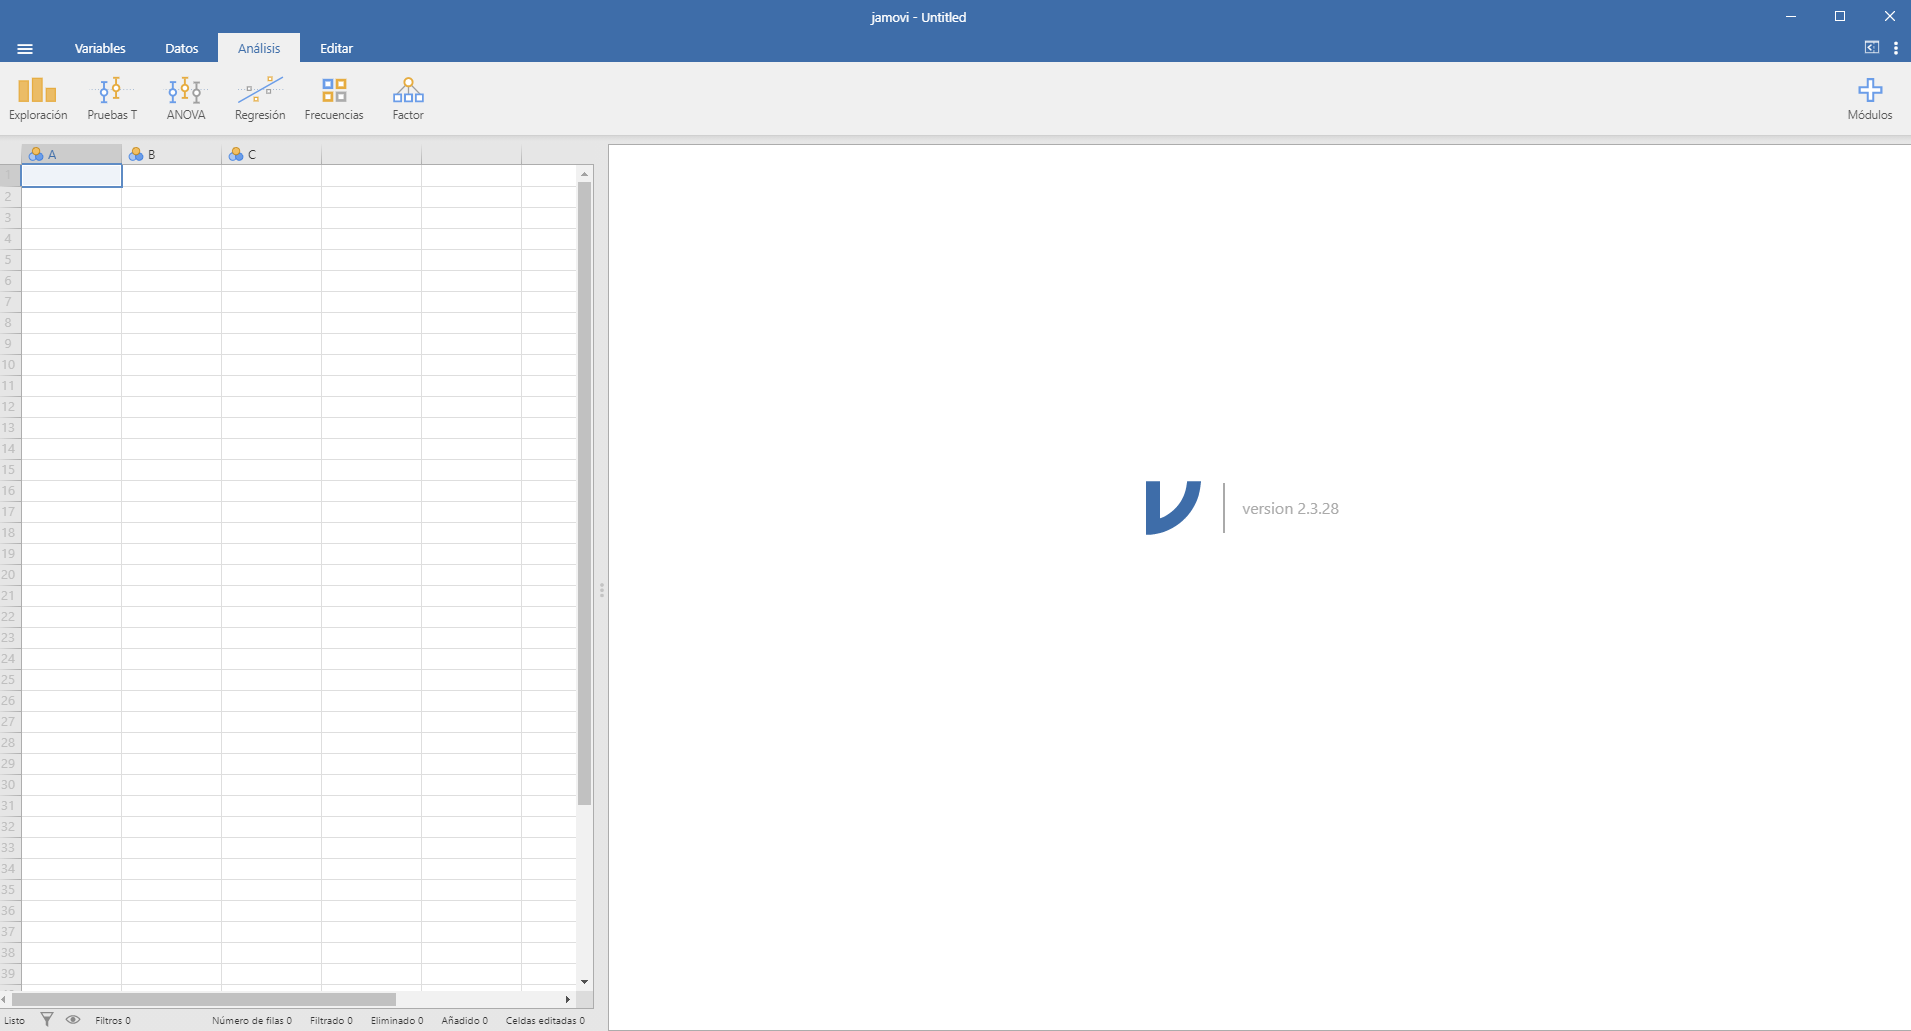
\includegraphics[width=0.8\textwidth,height=\textheight]{Figuras/JAM2.png}
\end{center}

\section{Matemáticas básicas}\label{matemuxe1ticas-buxe1sicas-1}

\subsection{Funciones lineales}\label{funciones-lineales}

En geometría analítica y álgebra elemental, una función lineal es una
función polinómica de primer grado, es decir, una función de una
variable (normalmente esta variable se denota con \(x\), que puede ser
escrita como la suma de términos de la forma \[f(x)=mx+b\] donde \(m\)
determina la pendiente o inclinación de la recta, y la constante \(b\)
determina el punto de corte de la recta con el eje vertical \(y\).

En Farmacia es útil observar la relación entre dosis y respuesta:

\begin{Shaded}
\begin{Highlighting}[]
\FunctionTok{library}\NormalTok{(tidyverse)}
\NormalTok{x }\OtherTok{=} \FunctionTok{seq}\NormalTok{(}\SpecialCharTok{{-}}\DecValTok{3}\NormalTok{,}\DecValTok{3}\NormalTok{)}
\NormalTok{y }\OtherTok{=} \DecValTok{2}\FloatTok{{-}0.5}\SpecialCharTok{*}\NormalTok{x}
\NormalTok{datos }\OtherTok{=} \FunctionTok{data.frame}\NormalTok{(x, y)}
\NormalTok{datos }\SpecialCharTok{\%\textgreater{}\%} \FunctionTok{ggplot}\NormalTok{(}\FunctionTok{aes}\NormalTok{(}\AttributeTok{x=}\NormalTok{x, }\AttributeTok{y=}\NormalTok{y))}\SpecialCharTok{+}
  \FunctionTok{geom\_line}\NormalTok{()}\SpecialCharTok{+}\FunctionTok{theme\_bw}\NormalTok{()}
\end{Highlighting}
\end{Shaded}

\begin{center}
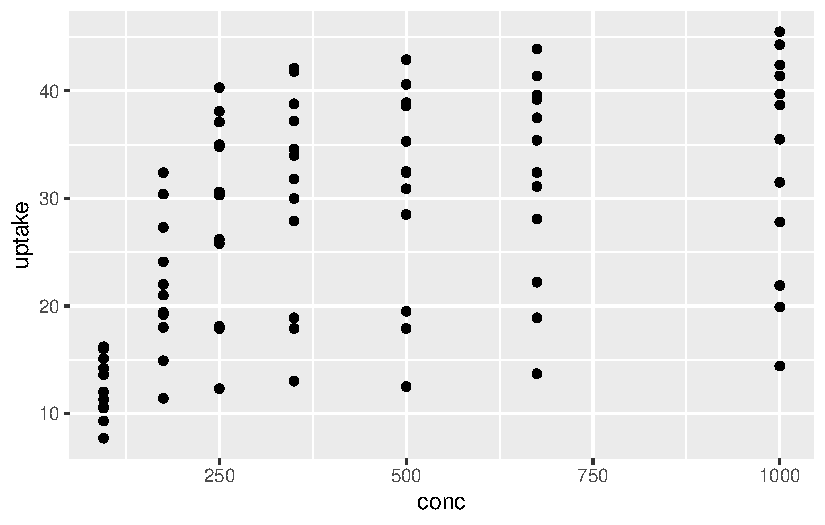
\includegraphics[width=0.6\textwidth,height=\textheight]{t2_MatesBasicas_files/figure-pdf/unnamed-chunk-1-1.pdf}
\end{center}

\subsection{Funciones exponenciales}\label{funciones-exponenciales}

Una función exponencial es una función matemática de la forma
\[f(x) = a \cdot b^x\],

donde:

\begin{itemize}
\tightlist
\item
  \(a\) es una constante que representa el valor inicial.
\item
  \(b\) es la base de la función exponencial.
\item
  \(x\) es la variable independiente.
\end{itemize}

Estas funciones son comunes en situaciones de crecimiento o
decrecimiento rápido, como el crecimiento poblacional, la desintegración
radiactiva, y el interés compuesto.

Consideremos una población de bacterias que se duplica cada hora. Si
inicialmente hay 100 bacterias, podemos modelar el crecimiento de la
población con la función exponencial:

\[P(t) = 100 \cdot 2^t\]

Aquí:

\begin{itemize}
\tightlist
\item
  \(P(t)\) es la población de bacterias en el tiempo \(t\) (en horas).
\item
  100 es el valor inicial ( \(a\) ).
\item
  2 es la base ( \(b\) ), ya que la población se duplica cada hora.
\end{itemize}

\begin{Shaded}
\begin{Highlighting}[]
\NormalTok{x }\OtherTok{=} \FunctionTok{seq}\NormalTok{(}\SpecialCharTok{{-}}\DecValTok{3}\NormalTok{,}\DecValTok{3}\NormalTok{, }\FloatTok{0.01}\NormalTok{)}
\NormalTok{y }\OtherTok{=} \DecValTok{100}\SpecialCharTok{*}\DecValTok{2}\SpecialCharTok{\^{}}\NormalTok{x}
\NormalTok{datos }\OtherTok{=} \FunctionTok{data.frame}\NormalTok{(x, y)}
\NormalTok{datos }\SpecialCharTok{\%\textgreater{}\%} \FunctionTok{ggplot}\NormalTok{(}\FunctionTok{aes}\NormalTok{(}\AttributeTok{x=}\NormalTok{x, }\AttributeTok{y=}\NormalTok{y))}\SpecialCharTok{+}
  \FunctionTok{geom\_line}\NormalTok{()}\SpecialCharTok{+}\FunctionTok{theme\_bw}\NormalTok{()}
\end{Highlighting}
\end{Shaded}

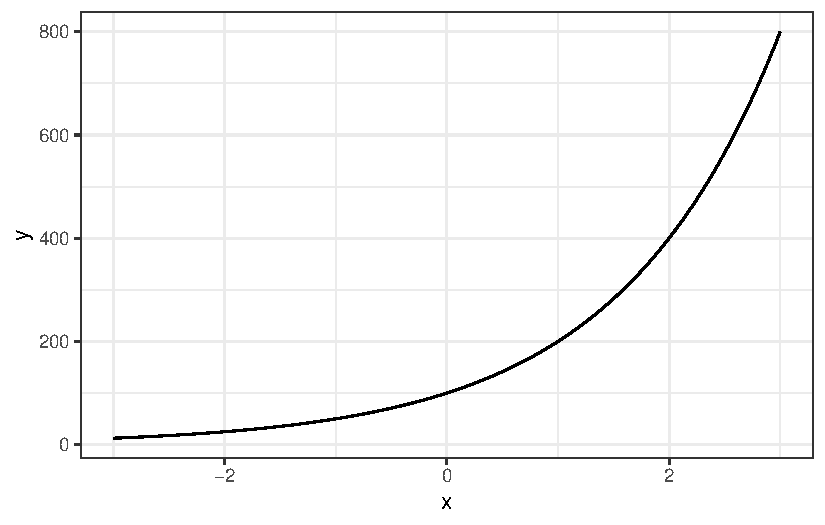
\includegraphics{t2_MatesBasicas_files/figure-pdf/unnamed-chunk-2-1.pdf}

\begin{Shaded}
\begin{Highlighting}[]
\NormalTok{x }\OtherTok{=} \FunctionTok{seq}\NormalTok{(}\SpecialCharTok{{-}}\DecValTok{3}\NormalTok{,}\DecValTok{3}\NormalTok{, }\FloatTok{0.01}\NormalTok{)}
\NormalTok{y }\OtherTok{=} \DecValTok{100}\SpecialCharTok{*}\FunctionTok{exp}\NormalTok{(x)}
\NormalTok{datos }\OtherTok{=} \FunctionTok{data.frame}\NormalTok{(x, y)}
\NormalTok{datos }\SpecialCharTok{\%\textgreater{}\%} \FunctionTok{ggplot}\NormalTok{(}\FunctionTok{aes}\NormalTok{(}\AttributeTok{x=}\NormalTok{x, }\AttributeTok{y=}\NormalTok{y))}\SpecialCharTok{+}
  \FunctionTok{geom\_line}\NormalTok{()}\SpecialCharTok{+}\FunctionTok{theme\_bw}\NormalTok{()}
\end{Highlighting}
\end{Shaded}

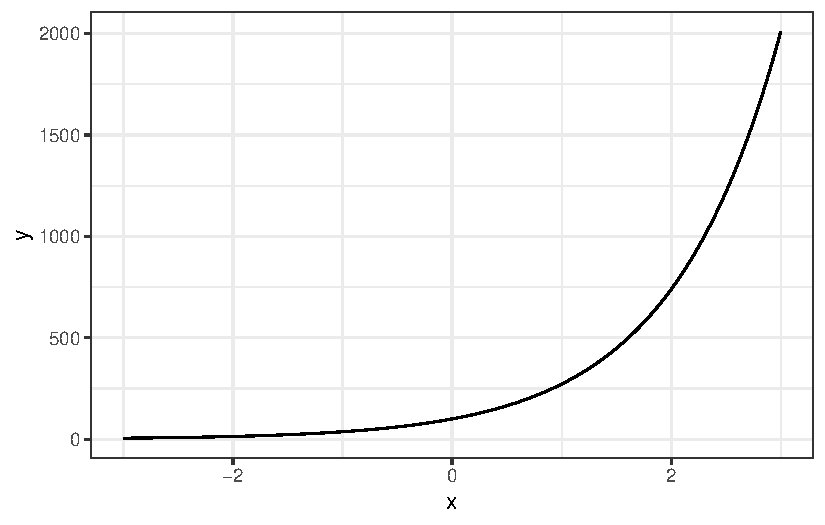
\includegraphics{t2_MatesBasicas_files/figure-pdf/unnamed-chunk-3-1.pdf}

\begin{tcolorbox}[enhanced jigsaw, colframe=quarto-callout-note-color-frame, coltitle=black, colback=white, toptitle=1mm, bottomrule=.15mm, bottomtitle=1mm, leftrule=.75mm, opacityback=0, rightrule=.15mm, titlerule=0mm, title=\textcolor{quarto-callout-note-color}{\faInfo}\hspace{0.5em}{Nota}, arc=.35mm, toprule=.15mm, left=2mm, opacitybacktitle=0.6, breakable, colbacktitle=quarto-callout-note-color!10!white]

Es muy importante reconocer el número \$e\approx \$ 2.7182818 como la
base más usada para tranajar con funciones exponenciales. Esto se debe a
la propiedad siguiente:
\[y = ab^x= e^{ln(ab^x)}=e^{xln b + a}=e^ae^{xln b}=\tilde{a}e^{\tilde{b}x}\]

\end{tcolorbox}

\subsection{Funciones logarítmicas}\label{funciones-logaruxedtmicas}

Una función logarítmica es la inversa de una función exponencial. Si
tenemos una función exponencial de la forma \(y=b^x\), donde \(b\) es la
base y \(x\) es el exponente, la función logarítmica correspondiente es
\(x=\log_b(y)\).

El logaritmo de un número \(y\) con base \(b\) es el exponente al cual
hay que elevar la base \(b\) para obtener \(y\). Matemáticamente, esto
se representa como:

\[log_b(y) = x \Leftrightarrow b^x = y\]

En el contexto de la farmacia, las bases más comunes son \(e\) (el
número de Euler, aproximadamente 2.718) y \(10\), dando lugar a los
logaritmos naturales (\(\ln(x)\)) y logaritmos en base 10
(\(\log_{10}(x)\)), respectivamente.

Las propiedades básicas de los logaritmos son especialmente útiles para
simplificar y resolver ecuaciones complejas:

\begin{enumerate}
\def\labelenumi{\alph{enumi}.}
\item
  \(\log_b(1) = 0\) para cualquier base \(b\).
\item
  Producto: \(\log_b(xy) = \log_b(x) + \log_b(y)\).
\item
  Cociente: \(\log_b(x/y) = \log_b(x) - \log_b(y)\).
\item
  Potencias: \(\log_b(x^p) = p \cdot \log_b(x)\).
\item
  Cambio de base: \(\log_b(x) = \frac{\log_a(x)}{\log_a(b)}\).
\end{enumerate}

Las funciones logarítmicas son ampliamente utilizadas en diversos
aspectos de la ciencia farmacéutica:

\begin{itemize}
\item
  \textbf{Farmacocinética}: Los logaritmos se utilizan para analizar
  cómo los medicamentos se distribuyen, metabolizan y eliminan en el
  cuerpo. Por ejemplo, la fórmula de eliminación de primer orden de un
  fármaco se representa mediante una función exponencial, y el tiempo de
  eliminación o la vida media se calculan usando logaritmos naturales.
\item
  \textbf{pH y Química Farmacéutica}: En química, los logaritmos son
  fundamentales para calcular el pH, que se define como el logaritmo
  negativo de la concentración de iones de hidrógeno:
  \[pH = -\log_{10}([H^+])\] Este concepto es clave para entender la
  estabilidad y solubilidad de los fármacos, así como para desarrollar
  soluciones que mantengan un pH constante en formulaciones
  farmacéuticas.
\item
  \textbf{Estudios de bioequivalencia}: Se comparan diferentes
  formulaciones de un mismo medicamento, el uso de logaritmos facilita
  el análisis de concentraciones plasmáticas a lo largo del tiempo,
  proporcionando una mejor comprensión de la absorción y distribución de
  los fármacos.
\item
  \textbf{Escalas y Dosificación}: Los logaritmos se utilizan para
  interpretar datos que cubren un amplio rango de valores, como las
  curvas dosis-respuesta, donde la relación entre la concentración de un
  medicamento y su efecto biológico es no lineal y puede ser mejor
  representada en una escala logarítmica.
\end{itemize}

Consideremos un ejemplo práctico en el que se necesita determinar el
tiempo necesario para reducir la concentración de un medicamento en
sangre a la mitad (vida media). Supongamos que la eliminación del
fármaco sigue una cinética de primer orden, es decir, la concentración
\[C(t) = C_0 \cdot e^{-kt}\] Donde \(C_0\) es la concentración inicial,
\(k\) es la constante de eliminación y \(t\) es el tiempo.

La vida media (\(t_{1/2}\)) se define como el tiempo necesario para que
la concentración del fármaco disminuya a la mitad de su valor inicial.
Entonces, para un fármaco con cinética de primer orden, la vida media se
calcula como:

\[t_{1/2} = \frac{\ln(2)}{k}\]

\subsection{Funciones polinómicas}\label{funciones-polinuxf3micas}

Una función polinomial de grado 2, también conocida como función
cuadrática, tiene la forma \(f(x) = ax^2 + bx + c\), donde:

\begin{itemize}
\tightlist
\item
  \(a\), \(b\) y \(c\) son constantes reales.
\item
  \(a\) es distinto de 0.
\end{itemize}

La gráfica de una función cuadrática es una parábola que puede abrirse
hacia arriba (si \(a\) es positivo) o hacia abajo (si \(a\) es
negativo).

\begin{Shaded}
\begin{Highlighting}[]
\NormalTok{x }\OtherTok{=} \FunctionTok{seq}\NormalTok{(}\SpecialCharTok{{-}}\DecValTok{3}\NormalTok{,}\DecValTok{3}\NormalTok{, }\FloatTok{0.01}\NormalTok{)}
\NormalTok{y }\OtherTok{=} \DecValTok{2}\FloatTok{+0.5}\SpecialCharTok{*}\NormalTok{x}\FloatTok{{-}0.4}\SpecialCharTok{*}\NormalTok{x}\SpecialCharTok{\^{}}\DecValTok{2}
\NormalTok{datos }\OtherTok{=} \FunctionTok{data.frame}\NormalTok{(x, y)}
\NormalTok{datos }\SpecialCharTok{\%\textgreater{}\%} \FunctionTok{ggplot}\NormalTok{(}\FunctionTok{aes}\NormalTok{(}\AttributeTok{x=}\NormalTok{x, }\AttributeTok{y=}\NormalTok{y))}\SpecialCharTok{+}
  \FunctionTok{geom\_line}\NormalTok{()}\SpecialCharTok{+}\FunctionTok{theme\_bw}\NormalTok{()}
\end{Highlighting}
\end{Shaded}

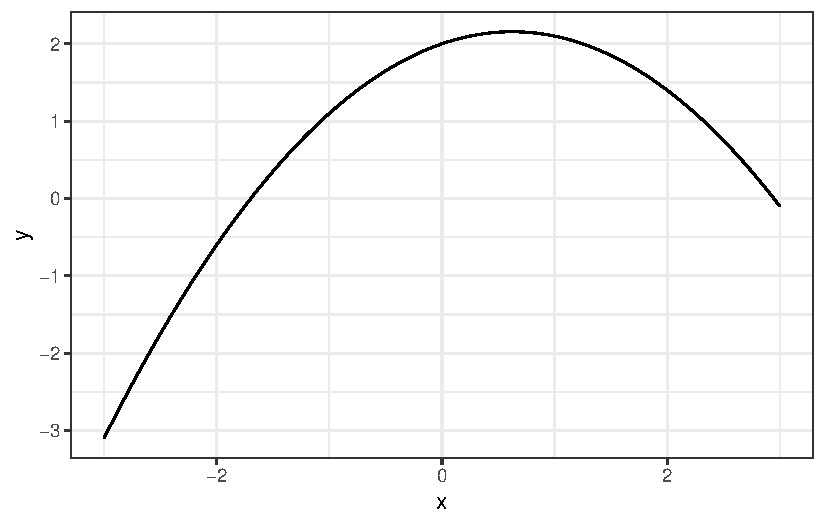
\includegraphics{t2_MatesBasicas_files/figure-pdf/unnamed-chunk-4-1.pdf}

\begin{Shaded}
\begin{Highlighting}[]
\NormalTok{x }\OtherTok{=} \FunctionTok{seq}\NormalTok{(}\SpecialCharTok{{-}}\DecValTok{10}\NormalTok{,}\DecValTok{10}\NormalTok{, }\FloatTok{0.01}\NormalTok{)}
\NormalTok{y }\OtherTok{=} \DecValTok{2}\FloatTok{+0.5}\SpecialCharTok{*}\NormalTok{x}\FloatTok{{-}0.4}\SpecialCharTok{*}\NormalTok{x}\SpecialCharTok{\^{}}\DecValTok{2} \SpecialCharTok{+}\FloatTok{0.5}\SpecialCharTok{*}\NormalTok{x}\SpecialCharTok{\^{}}\DecValTok{3}\FloatTok{{-}0.002}\SpecialCharTok{*}\NormalTok{x}\SpecialCharTok{\^{}}\DecValTok{5}
\NormalTok{datos }\OtherTok{=} \FunctionTok{data.frame}\NormalTok{(x, y)}
\NormalTok{datos }\SpecialCharTok{\%\textgreater{}\%} \FunctionTok{ggplot}\NormalTok{(}\FunctionTok{aes}\NormalTok{(}\AttributeTok{x=}\NormalTok{x, }\AttributeTok{y=}\NormalTok{y))}\SpecialCharTok{+}
  \FunctionTok{geom\_line}\NormalTok{()}\SpecialCharTok{+}\FunctionTok{theme\_bw}\NormalTok{()}
\end{Highlighting}
\end{Shaded}

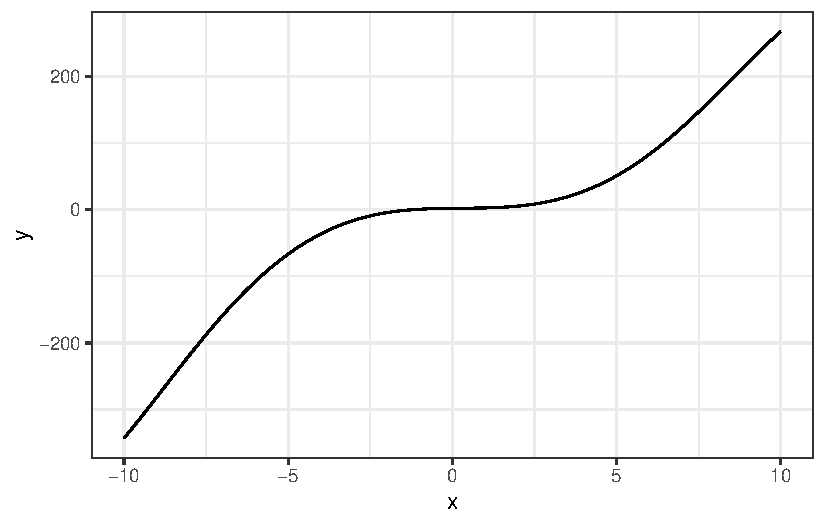
\includegraphics{t2_MatesBasicas_files/figure-pdf/unnamed-chunk-5-1.pdf}

\begin{tcolorbox}[enhanced jigsaw, colframe=quarto-callout-note-color-frame, coltitle=black, colback=white, toptitle=1mm, bottomrule=.15mm, bottomtitle=1mm, leftrule=.75mm, opacityback=0, rightrule=.15mm, titlerule=0mm, title=\textcolor{quarto-callout-note-color}{\faInfo}\hspace{0.5em}{Nota}, arc=.35mm, toprule=.15mm, left=2mm, opacitybacktitle=0.6, breakable, colbacktitle=quarto-callout-note-color!10!white]

Para recordar factorización, ¿qué sucede si graficamos la siguiente
función? \[y=(x-2)(x+1.5)(x-0.5)(x+3)(x+2)(x-4)\]

\end{tcolorbox}

\begin{Shaded}
\begin{Highlighting}[]
\NormalTok{x }\OtherTok{=} \FunctionTok{seq}\NormalTok{(}\SpecialCharTok{{-}}\DecValTok{3}\NormalTok{,}\DecValTok{4}\NormalTok{, }\FloatTok{0.01}\NormalTok{)}
\NormalTok{y }\OtherTok{=}\NormalTok{ (x}\DecValTok{{-}2}\NormalTok{)}\SpecialCharTok{*}\NormalTok{(x}\FloatTok{+1.5}\NormalTok{)}\SpecialCharTok{*}\NormalTok{(x}\FloatTok{{-}0.5}\NormalTok{)}\SpecialCharTok{*}\NormalTok{(x}\SpecialCharTok{+}\DecValTok{3}\NormalTok{)}\SpecialCharTok{*}\NormalTok{(x}\SpecialCharTok{+}\DecValTok{2}\NormalTok{)}\SpecialCharTok{*}\NormalTok{(x}\DecValTok{{-}4}\NormalTok{)}
\NormalTok{datos }\OtherTok{=} \FunctionTok{data.frame}\NormalTok{(x, y)}
\NormalTok{datos }\SpecialCharTok{\%\textgreater{}\%} \FunctionTok{ggplot}\NormalTok{(}\FunctionTok{aes}\NormalTok{(}\AttributeTok{x=}\NormalTok{x, }\AttributeTok{y=}\NormalTok{y))}\SpecialCharTok{+}
  \FunctionTok{geom\_line}\NormalTok{()}\SpecialCharTok{+}\FunctionTok{theme\_bw}\NormalTok{()}\SpecialCharTok{+}
  \FunctionTok{geom\_hline}\NormalTok{(}\AttributeTok{yintercept =} \DecValTok{0}\NormalTok{)}
\end{Highlighting}
\end{Shaded}

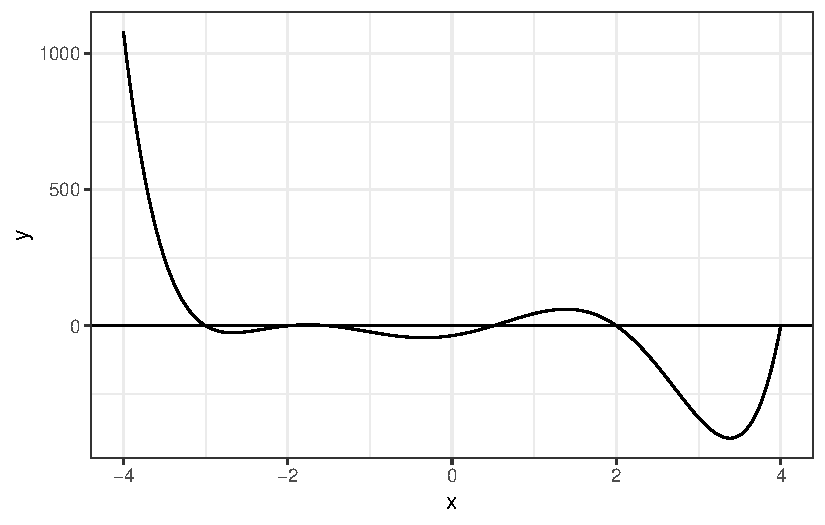
\includegraphics{t2_MatesBasicas_files/figure-pdf/unnamed-chunk-6-1.pdf}

\subsection{\texorpdfstring{{\emph{Práctica
1}}:}{Práctica 1:}}\label{pruxe1ctica-1}

\begin{itemize}
\item
  Formad grupos de 1, 2 o 3 integrantes.
\item
  Trabajaréis con los datos que aparecen en el
  \href{https://raw.githubusercontent.com/Cruzalirio/Ucentral/master/Bases/Global_Carbon_Budget_2018.csv}{enlace}.
  Abrimos el enlace y con click derecho --\textgreater{} Guardar como y
  seguimos las instrucciones.
\item
  Estos datos son tomados de la investigación sobre calentamiento global
  del \href{https://globalcarbonbudgetdata.org/latest-data.html}{Global
  Carbon Project}. Allí se encontrará más información por si os
  interesa. Vamos a introducir los gráficos de dispersión y la
  visualización de posibles relaciones entre variables cuantitativas.
\end{itemize}

Seguiremos los siguientes pasos.

\begin{itemize}
\item
  Con la opción abrir, importamos la base de datos en JAMOVI.
\item
  Verificamos que todas las variables estén cargadas
\item
  Reproduciremos esta gráfica de dispersión. ¿Cómo se realiza la
  gráfica? ¿De los tipos de funciones, cuál se ajustaria mejor?
\end{itemize}

\begin{center}
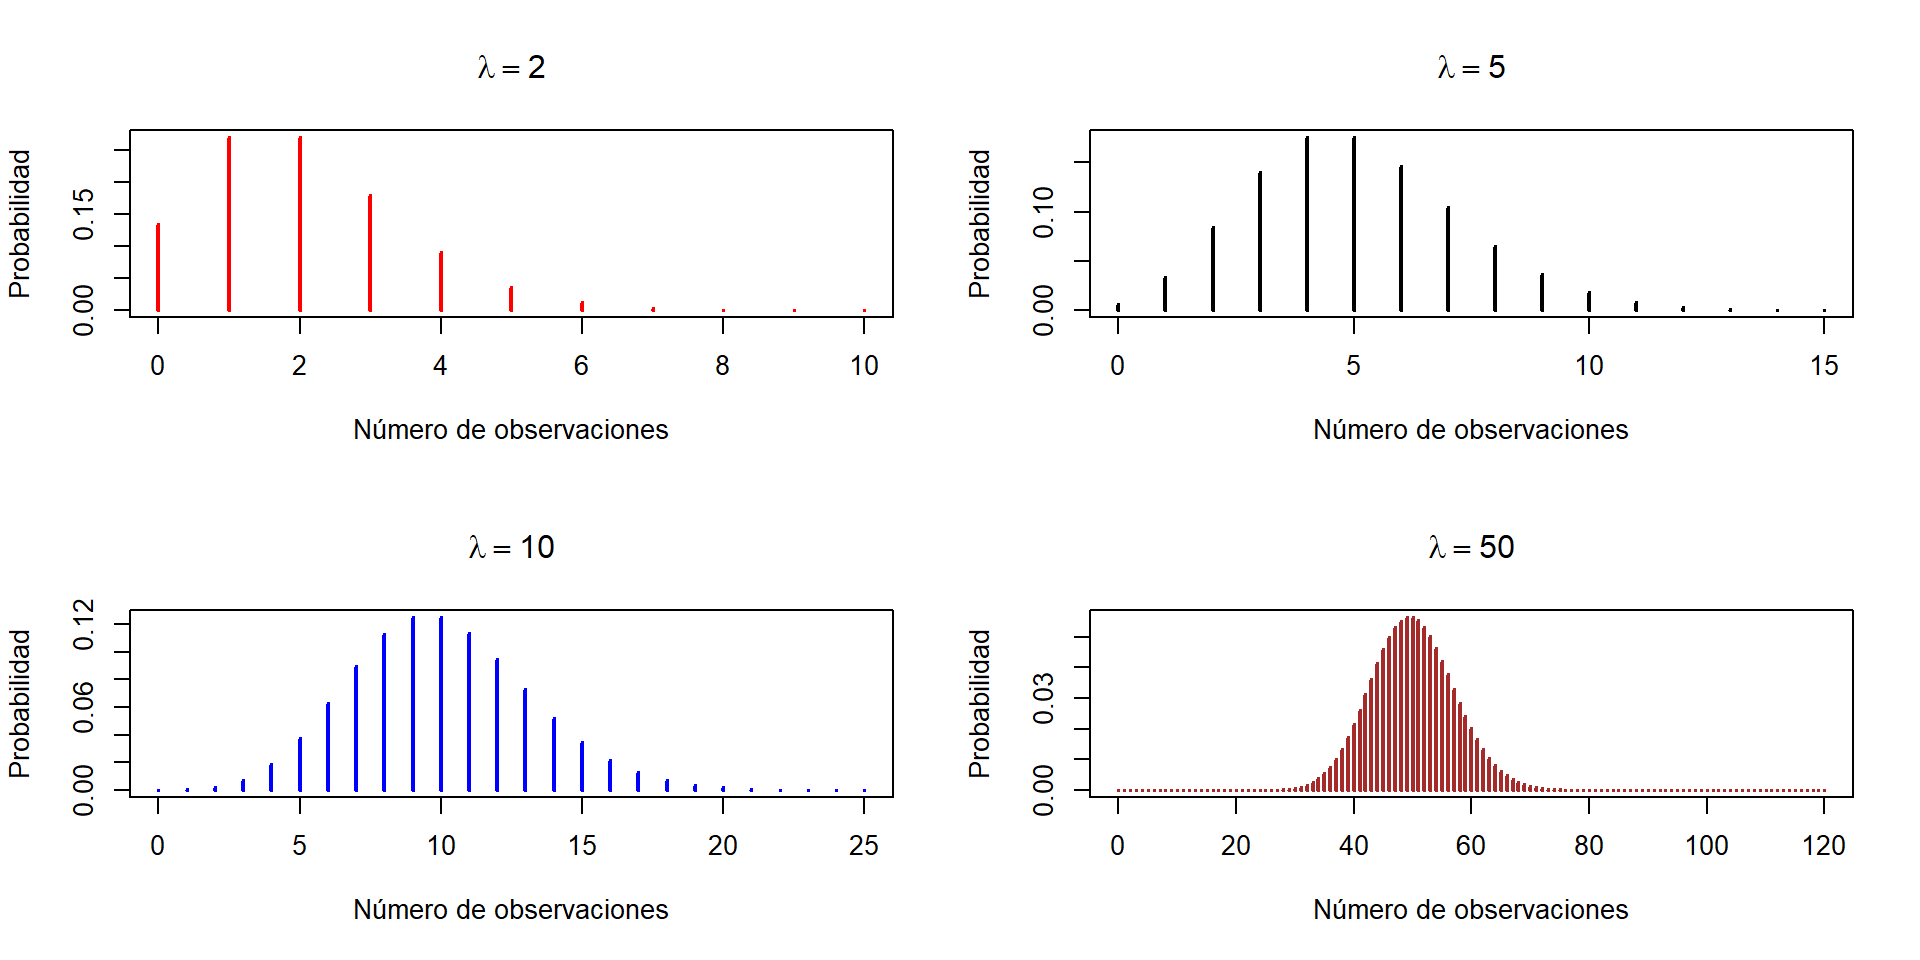
\includegraphics[width=0.6\textwidth,height=\textheight]{t2_MatesBasicas_files/figure-pdf/unnamed-chunk-7-1.pdf}
\end{center}

\begin{itemize}
\tightlist
\item
  Reproduciremos esta gráfica de dispersión. ¿Cómo se realiza la
  gráfica? ¿De los tipos de funciones, cuál se ajustaria mejor?
\end{itemize}

\begin{center}
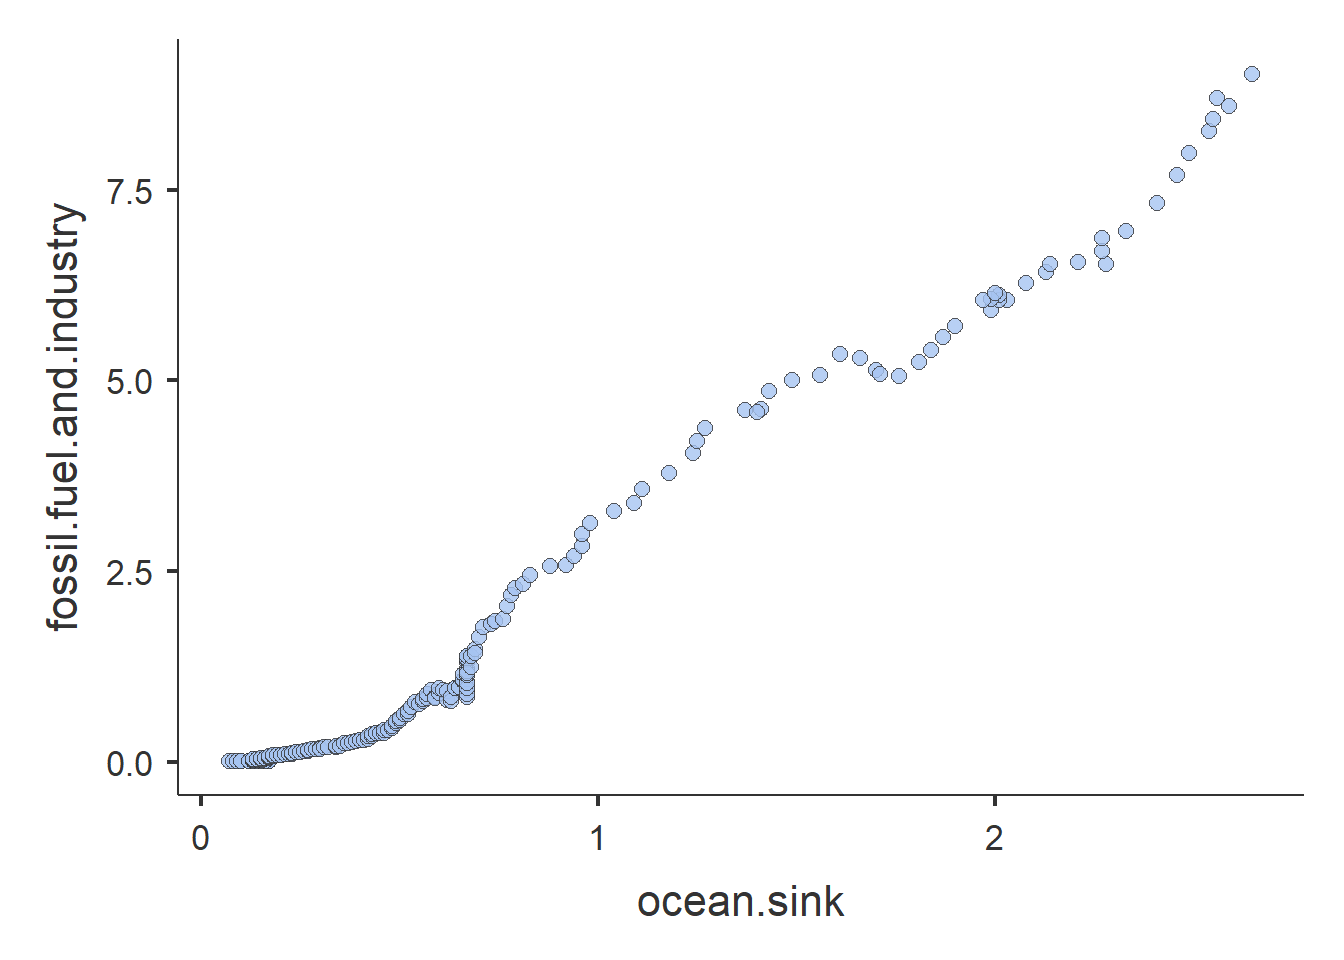
\includegraphics[width=0.6\textwidth,height=\textheight]{t2_MatesBasicas_files/figure-pdf/unnamed-chunk-8-1.pdf}
\end{center}

\begin{itemize}
\tightlist
\item
  Reproduciremos esta gráfica de dispersión. ¿Cómo se realiza la
  gráfica? ¿De los tipos de funciones, cuál se ajustaria mejor?
\end{itemize}

\begin{center}
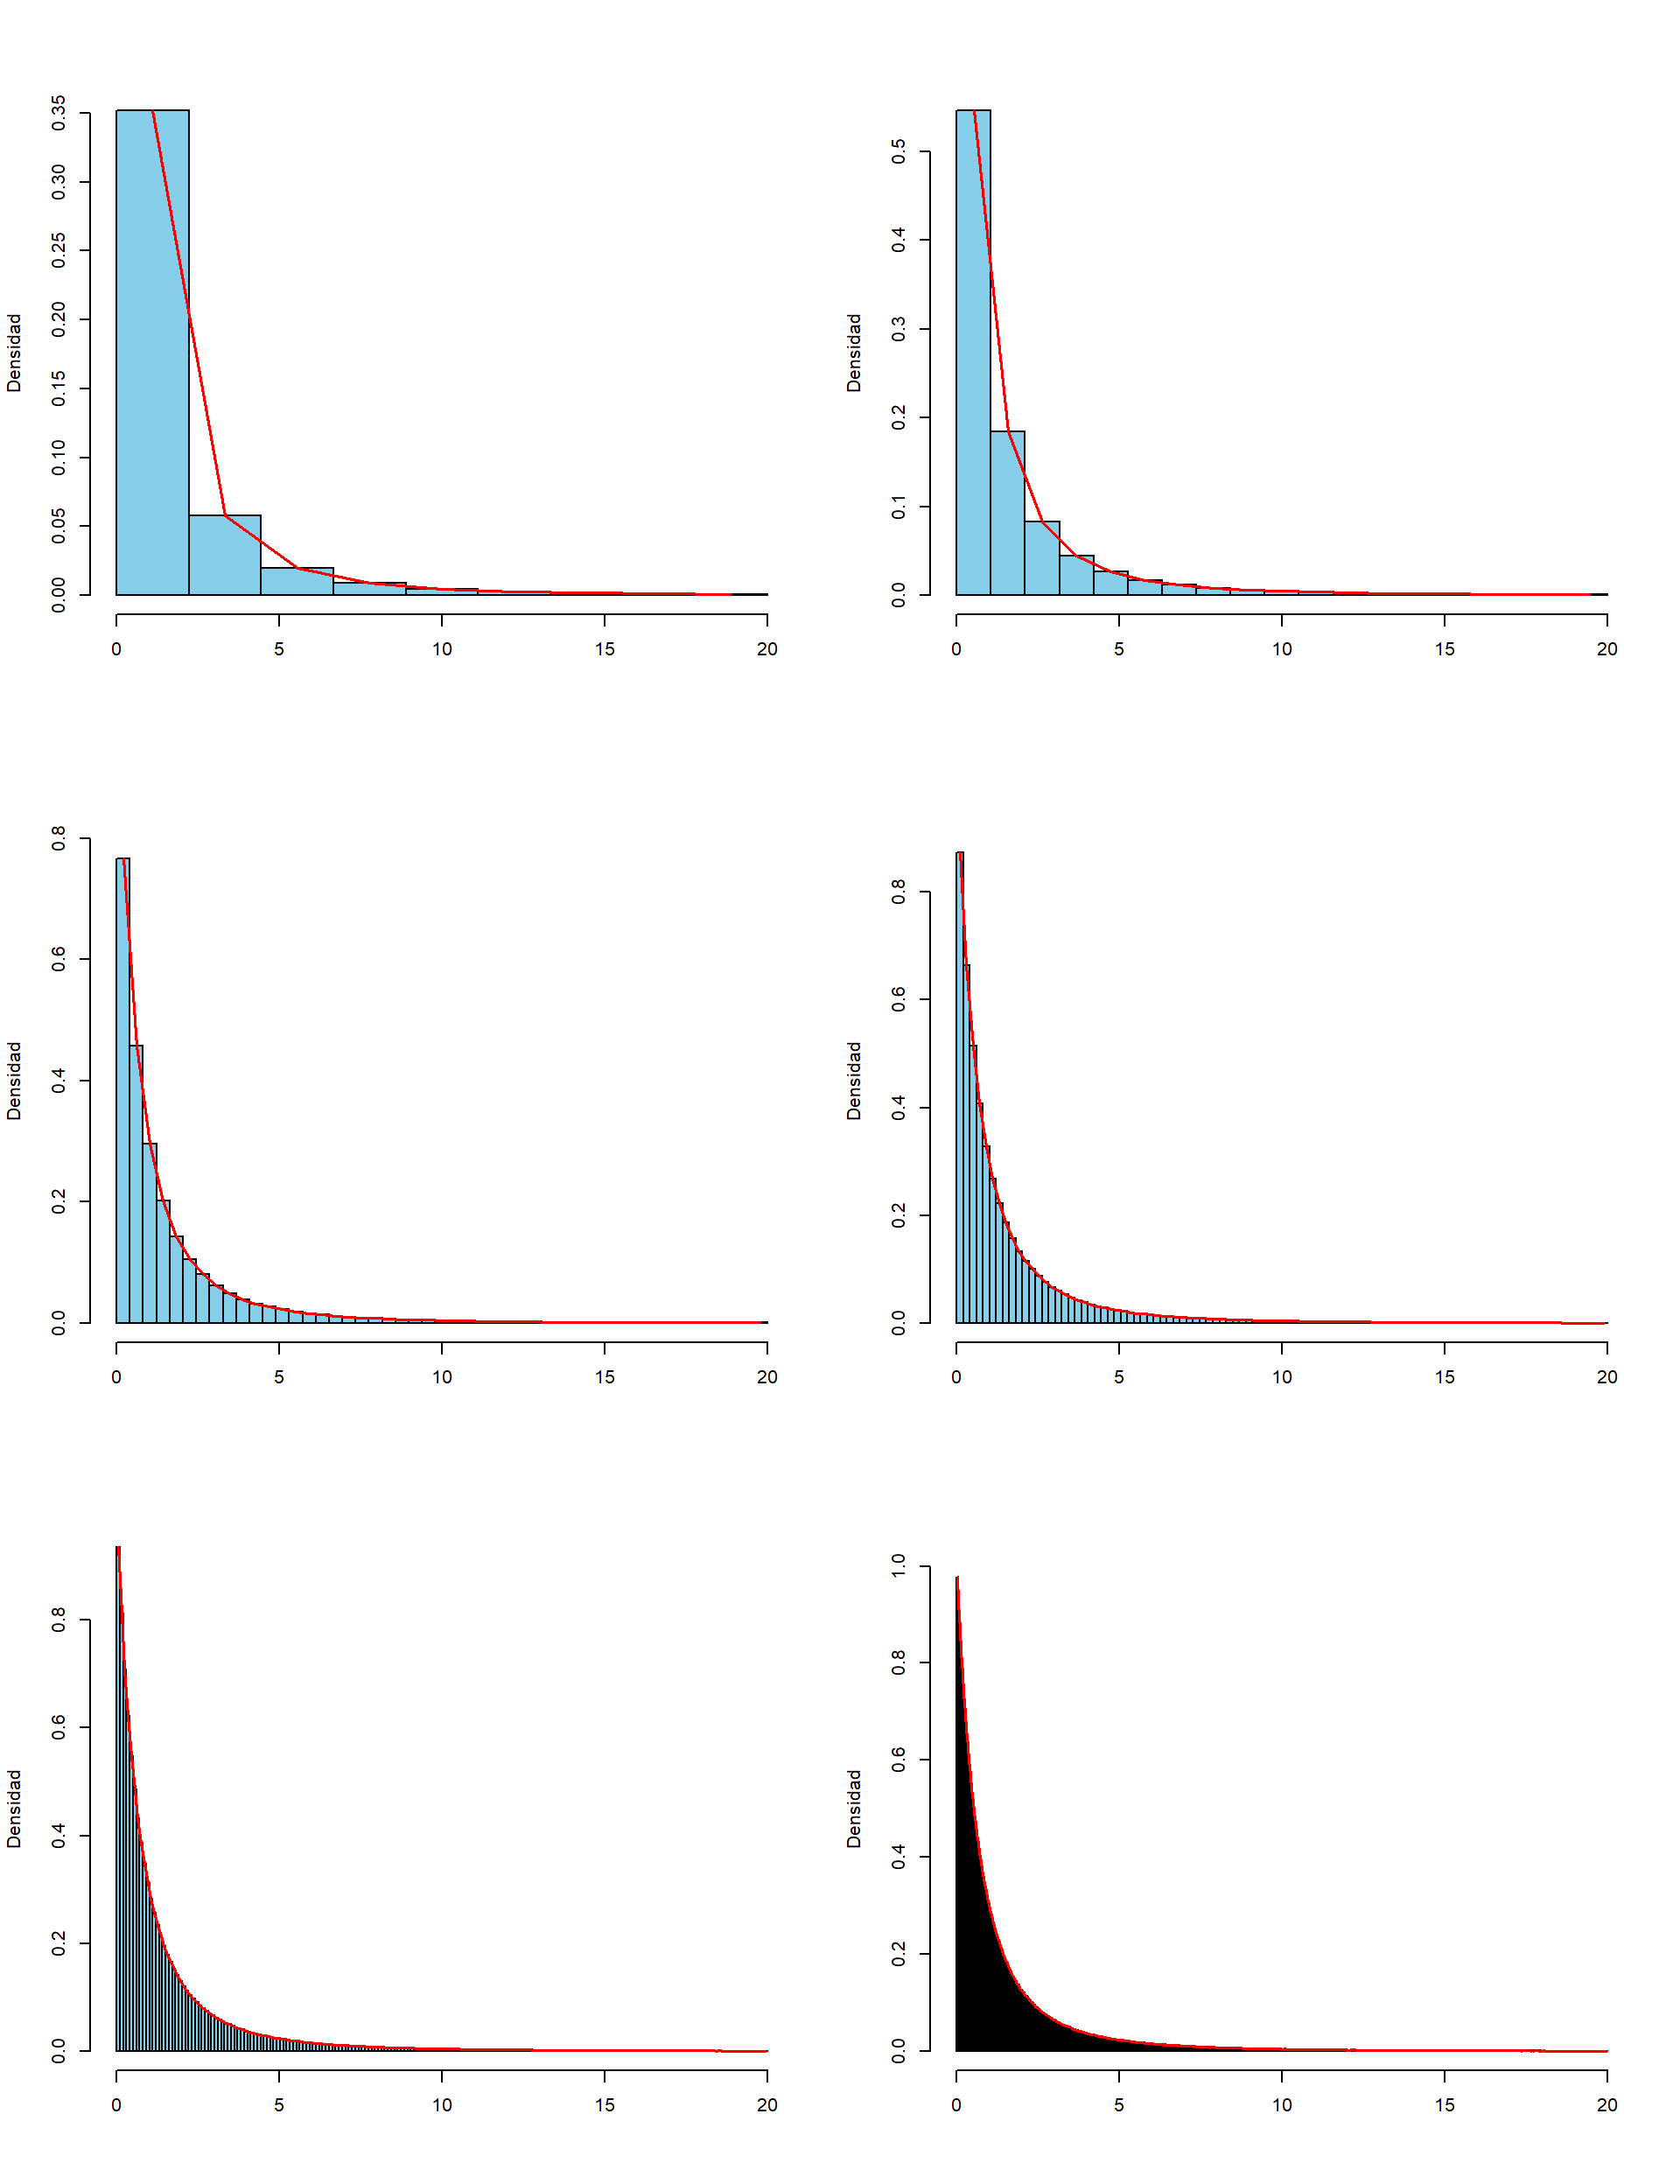
\includegraphics[width=0.6\textwidth,height=\textheight]{t2_MatesBasicas_files/figure-pdf/unnamed-chunk-9-1.pdf}
\end{center}

\begin{itemize}
\tightlist
\item
  Debéis exportar las gráficas en formato PDF.
\item
  Entregad el reporte en la tarea de Aula Digital disponible. Revisad la
  fecha en que cierra la tarea.
\end{itemize}

\bookmarksetup{startatroot}

\chapter{Representación gráfica y análisis de
Datos}\label{representaciuxf3n-gruxe1fica-y-anuxe1lisis-de-datos}

\section{La estadística y el método
científico}\label{la-estaduxedstica-y-el-muxe9todo-cientuxedfico}

\begin{itemize}
\item
  La ciencia avanza definiendo teorías que intentan explicar el mundo.
\item
  La comunidad científica elabora teorías/hipótesis que intentan
  explicar hechos que ocurren. Una hipótesis es científica si existe
  alguna manera de comprobar su veracidad.
\item
  Podemos diseñar experimentos para comprobar si se cumplen las
  afirmaciones de la teoría.
\item
  Como la naturaleza tiene un comportamiento con ``incertidumbre'', es
  decir, que si repetimos el experimento se obtienen resultados
  similares pero no idénticos, la estadística permite analizar estos
  resultados y ver si las desviaciones de la teoría son razonables o no.
\item
  Se ha definido estadística de muchas maneras. La que más nos gusta, y
  que está relaciona con la situación que acabamos de explicar, es que:
\end{itemize}

\begin{quote}
La \textbf{estadística} es la ciencia que permite adquirir conocimiento
generalizable a partir de datos.
\end{quote}

\begin{itemize}
\item
  La estadística ayuda en todas las fases del método científico:

  \begin{itemize}
  \item
    {\emph{Planteamiento del problema}}: Diseño de experimentos y
    encuestas, determinación del tamaño de la muestra y métodos de
    muestreo adecuados para garantizar que los datos recopilados sean
    representativos de la población objetivo.
  \item
    {\emph{Recopilación de datos}}: Proporciona herramientas para
    recopilar y organizar datos relevantes sobre el problema.
  \item
    {\emph{Análisis de datos}}: Aplicación de técnicas descriptivas
    (Análisis explorartorio de datos), así como técnicas inferenciales
    (contrastes de hipótesis, ajustes de modelos,etc) para sacar
    conclusiones sobre la población en función de la muestra recopilada.
  \item
    {\emph{Interpretación de resultados}}: Ayuda a los científicos a
    determinar si los resultados son estadísticamente significativos y
    si las conclusiones se pueden generalizar a la población más amplia.
  \item
    {\emph{Comunicación de hallazgos}}: La estadística se usa para
    comunicar los resultados de manera efectiva a través de gráficos,
    tablas y tests estadísticos. Esto es esencial para que otros
    investigadores puedan comprender y evaluar los resultados.
  \item
    {\emph{Reproducibilidad}}: Proporciona métodos estadísticos claros y
    transparentes, se permite que otros repitan los experimentos y
    análisis para verificar la validez de los hallazgos.
  \item
    {\emph{Toma de decisiones}}: En muchos campos científicos, los
    resultados estadísticos se utilizan para tomar decisiones
    importantes. Por ejemplo, en la medicina, la estadística se usa para
    evaluar la eficacia de tratamientos y tomar decisiones sobre su uso
    en la práctica clínica.
  \end{itemize}
\end{itemize}

En resumen, la estadística es una herramienta esencial que ayuda a
garantizar que la investigación científica sea rigurosa, confiable y
basada en evidencia sólida.

\section{Conceptos básicos}\label{conceptos-buxe1sicos}

\subsection{Estudio clínico}\label{estudio-cluxednico}

Un estudio clínico es un proceso cuyo objetivo es obtener evidencia
empírica sobre alguna cuestión. En el caso de los estudios que nos
ocupan en este curso, esta cuestión es, naturalmente, sobre algún
aspecto como la efectividad de un medicamento o algún tema de salud
pública.

\subsection{Unidad de observación}\label{unidad-de-observaciuxf3n}

En un estudio estadístico, la unidad de observación es, para
entendernos, el tipo de qué o de quiénes que son objeto de medición
durante la investigación. En los estudios médicos normalmente serán
personas, pero no siempre. Por ejemplo, pueden ser sucesos que les pasen
a personas, de manera que una misma persona pueda ser observada varias
veces: embarazos, operaciones quirúrgicas. Por ejemplo, podemos medir en
diferentes centros de educación primaria de una ciudad el gasto medio
diario en sus máquinas expendedoras de alimentos procesados y la
proporción de miopes entre sus alumnos, para estimar si hay alguna
relación entre el consumo de alimentos procesados y la miopía. Aquí, la
unidad de observación son los centros de educación primaria, no los
alumnos.

\subsection{Población y muestra}\label{poblaciuxf3n-y-muestra}

\begin{itemize}
\item
  \textbf{Población}: Es el conjunto de todas las unidades de
  observación sobre los que queremos conocer alguna información. Esta
  población puede estar perfectamente definida en un lugar y tiempo: por
  ejemplo, los empadronados en Mallorca a día de hoy. Pero normalmente
  su definición será difusa. Si, por ejemplo, queremos estimar algo
  sobre ``los españoles diabéticos mayores de 65 años'', ¿de quiénes
  estamos hablando exactamente? ¿De los que están vivos justo ahora? ¿De
  todos los que ha habido en España desde su fundación? ¿Incluimos los
  que aún no han nacido? ¿Qué hacemos con los que son diabéticos pero no
  han sido diagnosticados, ni lo serán nunca?
\item
  \textbf{Muestra}: Es un subconjunto de la población que se ha
  seleccionado para ser observado. La idea es que la muestra sea
  representativa de la población, de manera que los resultados obtenidos
  de la muestra puedan generalizarse a la población. En el ejemplo
  anterior, podríamos seleccionar una muestra de españoles diabéticos
  mayores de 65 años, y a partir de esta muestra intentar estimar alguna
  característica de la población de españoles diabéticos mayores de 65
  años.
\end{itemize}

\subsection{Tipos de estadística}\label{tipos-de-estaduxedstica}

En estadística, siempre se empieza obteniendo unos \textbf{datos} sobre
una muestra de una población. Bueno, en realidad, no se empieza
obteniendo los datos, sino planificando cuidadosamente cómo se van a
obtener.

Se \textbf{generaliza la información} que se ha obtenido sobre este
grupo de personas al total de la población. Y no se trata de trucos de
magia adivinatoria, sino de una \textbf{ciencia} cuya metodología ha
sido validada por medio de demostraciones matemáticas o, en el peor de
los casos, mediante simulaciones numéricas (el equivalente en
matemáticas de los experimentos en las otras ciencias).

Así pues, la situación de partida a la hora de aplicar técnicas
estadísticas es que disponemos de un conjunto de datos que describen
algunas características de un grupo de individuos. El análisis
estadístico de estos datos puede ser entonces de dos tipos básicos:

\begin{itemize}
\item
  \textbf{Análisis exploratorio de datos}, cuando nuestro objetivo sea
  simplemente resumir, representar y explicar los datos concretos de los
  que disponemos. La \textbf{estadística descriptiva} es el conjunto de
  técnicas que se usan con este fin.
\item
  \textbf{Análisis inferencial}, si nuestro objetivo es deducir
  (\textbf{inferir}), a partir de estos datos, información significativa
  sobre el total de la población de interés. Las técnicas que se usan en
  este caso forman la \textbf{estadística inferencial}.
\end{itemize}

\begin{center}
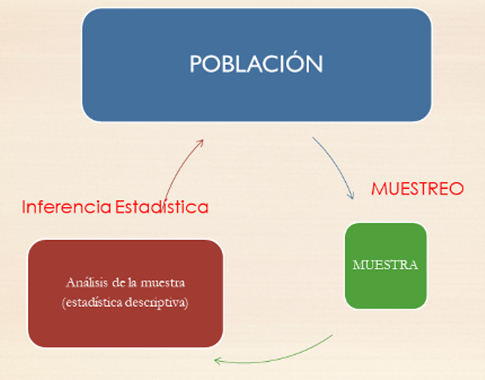
\includegraphics[width=0.8\textwidth,height=\textheight]{Figuras/muestreo_inferencia.png}
\end{center}

Ambos tipos de análisis están relacionados. Por un lado, porque es
conveniente (obligatorio, en nuestra opinión) empezar cualquier análisis
inferencial dando un vistazo a los datos que se usarán.

Por otro, porque muchas técnicas descriptivas permiten estimar
propiedades de la población de la que se ha extraído la muestra. Por
citar un ejemplo, la media aritmética de las alturas de un grupo de
individuos nos da un valor más o menos representativo de sus alturas,
pero también sirve para \emph{estimar} la altura media de los individuos
de la población total.

La estadística inferencial entra en juego cuando se quiere obtener
información sobre una población y no se puede acceder a todos sus
integrantes. Si por ejemplo queremos conocer la altura media de los
estudiantes matriculados en esta asignatura de la UIB en este curso, en
principio no necesitamos para nada la estadística inferencial. Sois
pocos, os mediríamos a todos y calcularíamos la media. En todo caso,
usaríamos técnicas de estadística descriptiva para arropar este valor
representando la distribución de vuestras alturas de manera adecuada.

Pero si quisiéramos conocer la altura media de los mallorquines entre 18
y 25 años, sería muy complicado medirlos a todos. Entonces, lo que
haríamos sería tomar una muestra representativa de esta población,
medirlos y a partir de sus alturas estimar dicha altura media.
Naturalmente, lo más seguro es que de esta manera no obtuviéramos el
valor exacto de la altura media de los mallorquines de 18 años, nos
tendríamos que conformar con obtener una aproximación dentro de un
cierto margen de error y determinar la probabilidad de acertar con
nuestra estimación y este margen de error. La estadística inferencial es
la que nos permite acotar el error que podamos haber cometido y calcular
la probabilidad de cometerlo, incluyendo la metodología que tendríamos
que haber usado para tomar la muestra en primer lugar.

\subsection{Tipos de estudios}\label{tipos-de-estudios}

Podemos clasificar los estudios clínicos de diferentes maneras:

\begin{itemize}
\item
  Según su \textbf{intención}:

  \begin{itemize}
  \item
    \textbf{Descriptivos}: Se limitan a describir las características de
    los individuos de la muestra.
  \item
    \textbf{Analíticos}: Intentan inferir conclusiones sobre el total de
    la población.
  \end{itemize}
\item
  Según el \textbf{papel jugado por el investigador}:

  \begin{itemize}
  \item
    \textbf{Observacionales}: El investigador se limita a recoger datos,
    sin ejercer ninguna influencia planificada sobre los acontecimientos
    que generan dichos datos.
  \item
    \textbf{Intervencionista}: El investigador lleva a cabo una
    intervención en los participantes (por ejemplo, les administra
    tratamientos farmacológicos o recomienda cambios de comportamiento)
    de manera planificada y con el objetivo de generar los datos que
    permitan evaluar el efecto de dicha intervención.
  \end{itemize}
\item
  Según el \textbf{lapso de tiempo} sobre el que se recoge la
  información:

  \begin{itemize}
  \item
    \textbf{Transversales}: Se recoge información sobre un solo momento.
  \item
    \textbf{Longitudinales}: Se recoge información sobre varios momentos
    de tiempo y se estudian los cambios producidos entre los mismos.

    A su vez, estos últimos suelen dividirse en:

    \begin{itemize}
    \item
      \textbf{Prospectivos}: Se recoge información en un momento
      concreto (normalmente, al inicio del estudio) y en momentos
      posteriores.
    \item
      \textbf{Retrospectivos}: Se recoge información en un momento
      concreto (de nuevo, normalmente, al inicio del estudio) y sobre
      momentos anteriores.
    \end{itemize}
  \end{itemize}
\end{itemize}

Combinando los tipos de estudio según el papel jugado por el
investigador y según el lapso de tiempo sobre el que se recoge la
información, tenemos estudios:

\begin{itemize}
\tightlist
\item
  Observacionales transversales
\item
  Observacionales prospectivos
\item
  Observacionales retrospectivos
\item
  Intervencionistas transversales
\item
  Intervencionistas prospectivos
\item
  Intervencionistas retrospectivos
\end{itemize}

Acabamos de ver que hay estudios intervencionistas prospectivos. ¿Los
hay de las otras cinco clases de estudios de esta lista, o hay algún par
de características que es imposible que se den simultáneamente?

\bookmarksetup{startatroot}

\chapter*{Referencias}\label{referencias}
\addcontentsline{toc}{chapter}{Referencias}

\markboth{Referencias}{Referencias}

\phantomsection\label{refs}
\begin{CSLReferences}{0}{1}
\end{CSLReferences}

\begin{itemize}
\item
  Bolton, S., \& Bon, C. B. (2010). Pharmaceutical Statistics: Practical
  and Clinical Applications (5th ed.). CRC Press.
\item
  Martínez González, M., Sánchez Villegas, A., \& Faulín Fajardo, J.
  (2020). Bioestadística Amigable. CRC Press.
\end{itemize}



\end{document}
